			\subsubsection{Wydajność}
			\par Celem przeprowadzenia analizy wydajnościowej systemu należy sprecyzować komponenty, z jakich składać się musi system. Zostanie to zrealizowane poprzez rozszerzenie schematu \ref{basic_comp} o pozostałe konieczne do działania komponenty systemu.
		
			\begin{figure}[H]
				\centering
				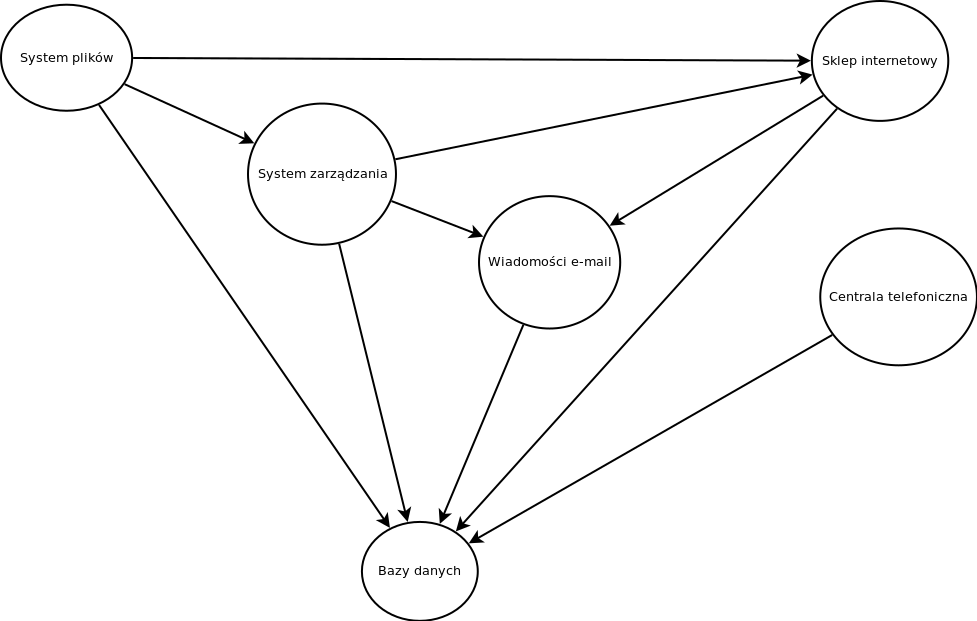
\includegraphics[scale=0.45]{extended_comp}
				\caption{Rozszerzony diagram komponentów systemu}
			\end{figure}
		
			Diagram komponentów \ref{basic_comp} został rozszerzony o centralę telefoniczną oraz system plików. Centrala telefoniczna służy obsłudze przychodzących i wychodzących rozmów telefonicznych, natomiast system plików jest komponentem służącym przechowywaniu danych z wszystkich pozostałych elementów systemu. 
		
			\par Wykorzystując abstrakcyjny schemat komponentów systemu można utworzyć system komputerowy realizujący założona funkcjonalność. Na podstawie schematu \ref{extended_comp} można przygotować listę programowych komponentów systemu komputerowego. Z powyższego schematu wynika wprost, że system komputerowy musi składać się z następujących komponentów programowych: systemu baz danych, systemu plików, centrali telefonicznej, systemu wiadomości e-mail, systemu zarządzania i sklepu internetowego. Ponadto system komputerowy, aby spełniać wymogi realizowanych na nim działań musi zawierać również system DNS (z ang. Domain Resolve System) czyli system nazw domenowych, odpowiedzialny za tłumaczenie adresów domen na adresy IP. Jest to wymóg rfc1035, aby móc przechowywać domenę. 
			
			\par Korzystając z poprzedniego paragrafu można ustalić podstawowy schemat sieci firmowej. System zarządzania oraz sklep internetowy muszą znajdować się na serwerze www, oprogramowanie to jest odpowiedzialne za wygenerowanie dynamicznej strony internetowej na żądanie klienta lub pracownika sklepu. Następnym elementem będzie serwer wiadomości e-mail odpowiedzialny za komunikację elektroniczną. Kolejnym elementem systemu jest serwer centrali telefonicznej odpowiedzialny za połączenia przychodzące i wychodzące. Elementem wymaganym przez poprzednie składowe systemu jest serwer baz danych, na którym zapisywane będą dane pochodzące z poprzednich serwerów. Przedostatnim elementem jest serwer sieciowego systemu plików, na którym zapisywane będą dane pochodzące z serwera baz danych oraz wszystkie pozostałe pliki. Ostatnim elementem będą dwa serwery DNS, które są wymagane do samodzielnego przechowywania domeny.
			
		
			Lista serwerów potrzebnych do zrealizowania założeń obsługi klienta i funkcjonowania firmy: 
			\begin{itemize}
				\item Dwa serwery DNS
				\item Serwer wiadomości e-mail
				\item Serwer baz danych
				\item Centrala telefoniczna
				\item Serwer sieciowego systemu plików
				\item Serwer www
			\end{itemize}
		
			Na podstawie powyższej listy można przygotować podstawowy schemat systemu komputerowego. Należy rozszerzyć go o wcześniej nie wspomniane elementy jakimi są router i most sieciowy. Router'em nazywamy urządzenie komputerowe odpowiadające za trasowanie informacji na poziomie programowym do odpowiednich elementów systemu. Natomiast most sieciowy jest elementem spajającym wszystkie elementy sieci w spójną całość.
		
			\begin{figure}[H]
				\centering
				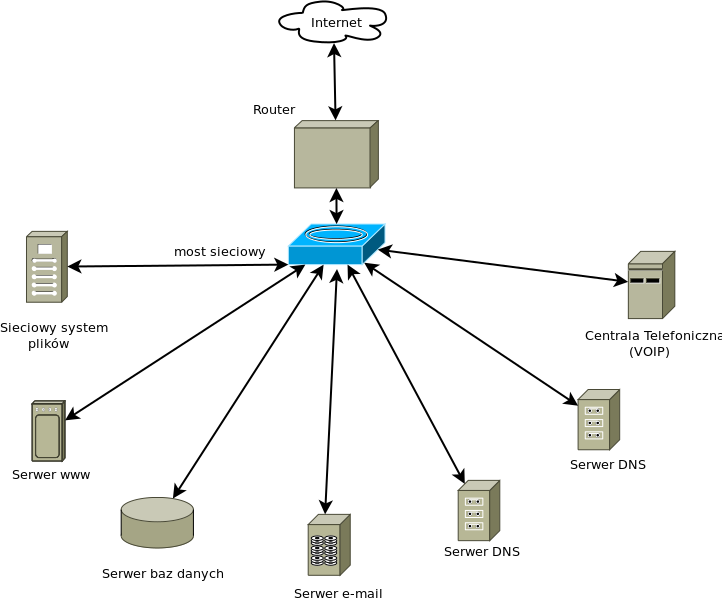
\includegraphics[scale=0.45]{Basic}
				\caption{Podstawowy schemat sieci}
				\label{basic_net}
			\end{figure}
			
			\par Serwery przedstawione na schemacie \ref{basic_net} mogą być komputerami fizycznymi lub komputerami wirtualnymi. Technologia wirtualizacji w systemach serwerowych pozwala utworzyć na komputerze fizycznym komputery wirtualne korzystające z jego zasobów. Innymi słowy na jednym fizycznym komputerze można uruchomić kilka komputerów wirtualnych. 
		
		\paragraph{Zasoby sprzętowe}
			\par Korzystając z dobrodziejstwa wirtualizacji, sieć ze schematu \ref{basic_net} można uruchomić na jednym komputerze fizycznym. Należałoby określić zasoby sprzętowe tego komputera, dokonując analizy wydajnościowej.
		
			\par Na podstawie analizy niezawodności popartej rachunkiem prawdopodobieństwa udało się ustalić diagram sieci idealnej. Separacja elementów sieci przyniosła spodziewane rezultaty w postaci obniżenia prawdopodobieństwa awarii uniemożliwiającej funkcjonowanie systemu w cyklu 3 letnim z 18\% do 3.24\%. Pociąga ona za sobą jednak konsekwencje w postaci podniesienia prawdopodobieństwa wystąpienia jakiejkolwiek awarii, co logicznie związane jest ze zwiększeniem ilości urządzeń z jakich składa się system. Uzasadnione będzie znalezienie tu kompromisu pomiędzy ceną i aspektami niezawodności. Na podstawie powyższych rozważań można przygotować ostateczny diagram sieci firmowej.
		
		\begin{figure}[H]
			\centering
			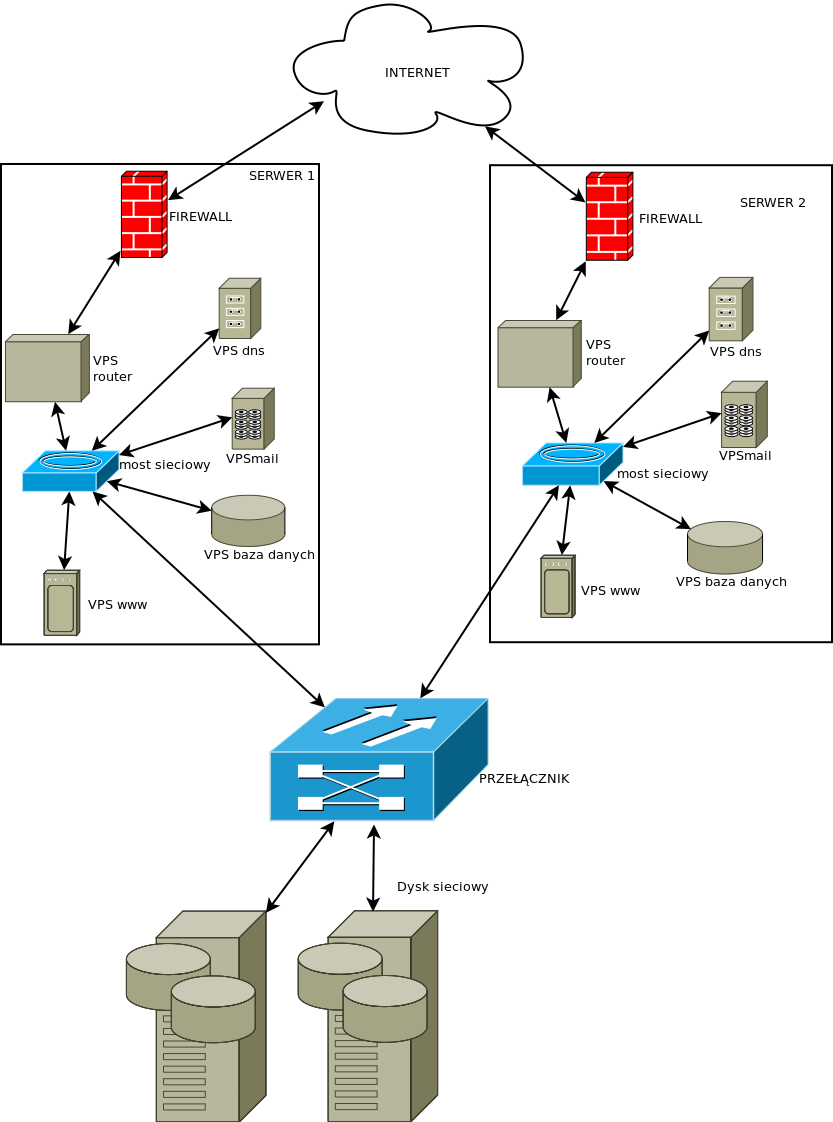
\includegraphics[scale=0.45]{Diagram2}
			\caption{Ostateczny diagram sieci}
			\label{net_real}
		\end{figure}
 
 
